%%%%%%%%%%%%%%%%%%%%%%%%%%%%%%%%%%%%%%%%%
% Friedrich M. Grabner
% CFD Coursework 1
%
%%%%%%%%%%%%%%%%%%%%%%%%%%%%%%%%%%%%%%%%%

%----------------------------------------------------------------------------------------
%	PACKAGES AND DOCUMENT CONFIGURATIONS
%----------------------------------------------------------------------------------------
\documentclass[10pt, a4paper]{article}
\usepackage{amsmath, amsthm, amssymb}
\usepackage{graphicx} % Required for the inclusion of images
\usepackage{natbib} % Required to change bibliography style to APA
\usepackage{nomencl}
\usepackage{setspace}
\usepackage{geometry} 
\usepackage{hyperref}
\usepackage{subcaption}

\geometry{a4paper,total={170mm,257mm},left=20mm,top=20mm}



\setlength\parindent{5pt} % Removes all indentation from paragraphs
\graphicspath{{./images/}}
\DeclareGraphicsExtensions{.pdf,.PDF,.jpg,.JPG,.bmp,.png,.eps,.EPS}

%\usepackage{times} % Uncomment to use the Times New Roman font

\input{/home/fmg215/Documents/latex/symbols.tex}
%----------------------------------------------------------------------------------------
%	DOCUMENT INFORMATION
%----------------------------------------------------------------------------------------
\newcommand*{\plogo}{\fbox{$\mathcal{PL}$}}

\newcommand*{\titleGM}{\begingroup % Create the command for including the title page in the document
\hbox{ % Horizontal box
\hspace*{0.2\textwidth} % Whitespace to the left of the title page
\rule{1pt}{\textheight} % Vertical line
\hspace*{0.05\textwidth} % Whitespace between the vertical line and title page text
\parbox[b]{0.75\textwidth}{ % Paragraph box which restricts text to less than the width of the page

{\noindent\Huge\bfseries CFD Assignment 2 \\[0.5\baselineskip] AEM-ADV19}\\[2\baselineskip] % Title
{\Large \textsc{Friedrich M. Grabner - 01220997}}\\[4\baselineskip] % Tagline or further description
{\large } % Author name

\vspace{0.5\textheight} % Whitespace between the title block and the publisher
{\noindent Imperial College London - Department of Aeronautics}\\[\baselineskip] % Publisher and logo
}}
\endgroup}
%----------------------------------------------------------------------------------------
%	TITLE PAGE
%----------------------------------------------------------------------------------------
\begin{document}
\titleGM
%----------------------------------------------------------------------------------------
%	QUESTION 1
%----------------------------------------------------------------------------------------
\section{}
\textbf{Run a first simulation with $Re = 200$ (line 646 of the \url{2D_compressible.f90} file) and $n_x \times n_y = 129 \times 129$ for $n_t = 10000$ time steps with a second order Adams-Bashforth scheme (itemp=1) and a CFL equal to 0.25. Generate 4 visualisations of the vorticity field for $n_t = 2500, 5000, 7500, 10000$. Briefly comment on the results in less than 100 words. (Note : The code should be configured for this question, no changes are needed).}

\begin{figure}[htb!]
\centering
\begin{subfigure}{.5\textwidth}
  \centering
  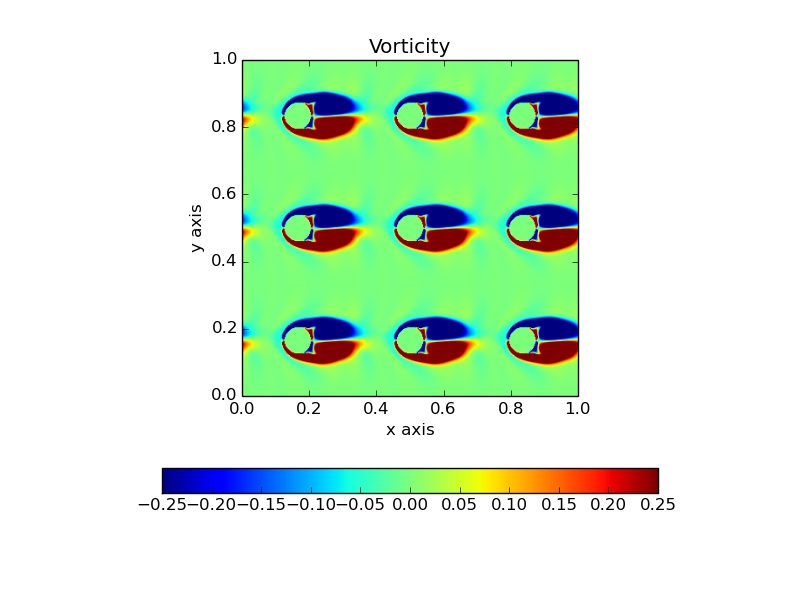
\includegraphics[width=1.1\linewidth, clip=true, trim=1cm 1cm 1cm 1cm]{q1_0001}
  \caption{$n_t = 2500$}
  \label{fig:sub1}
\end{subfigure}%
\begin{subfigure}{.5\textwidth}
  \centering
  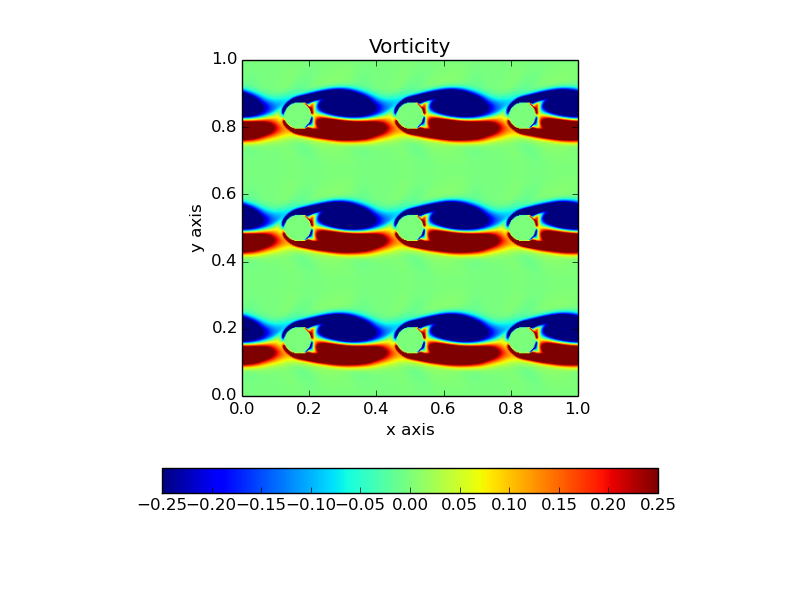
\includegraphics[width=1.1\linewidth, clip=true, trim=1cm 1cm 1cm 1cm]{q1_0002}
  \caption{$n_t = 5000$}
  \label{fig:sub2}
\end{subfigure}
\newline
\begin{subfigure}{.5\textwidth}
  \centering
  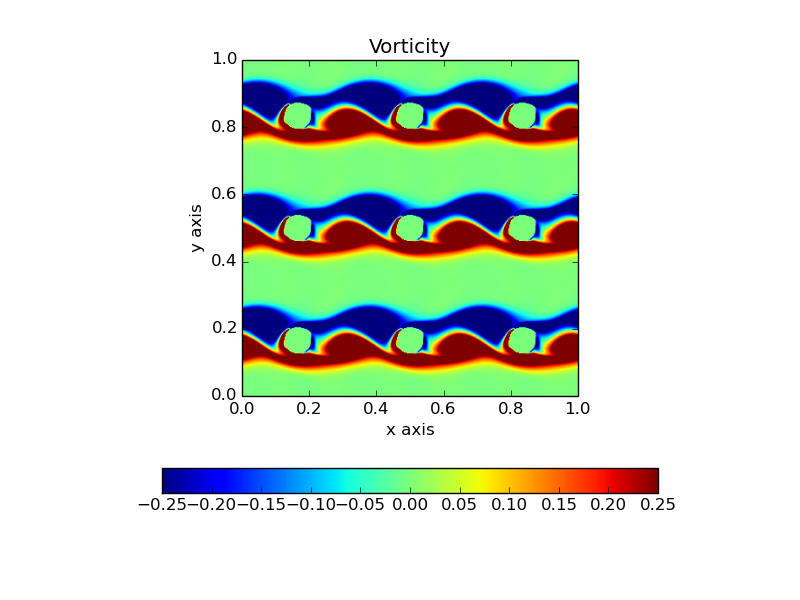
\includegraphics[width=1.1\linewidth, clip=true, trim=1cm 1cm 1cm 1cm]{q1_0003}
  \caption{$n_t = 7500$}
  \label{fig:sub1}
\end{subfigure}%
\begin{subfigure}{.5\textwidth}
  \centering
  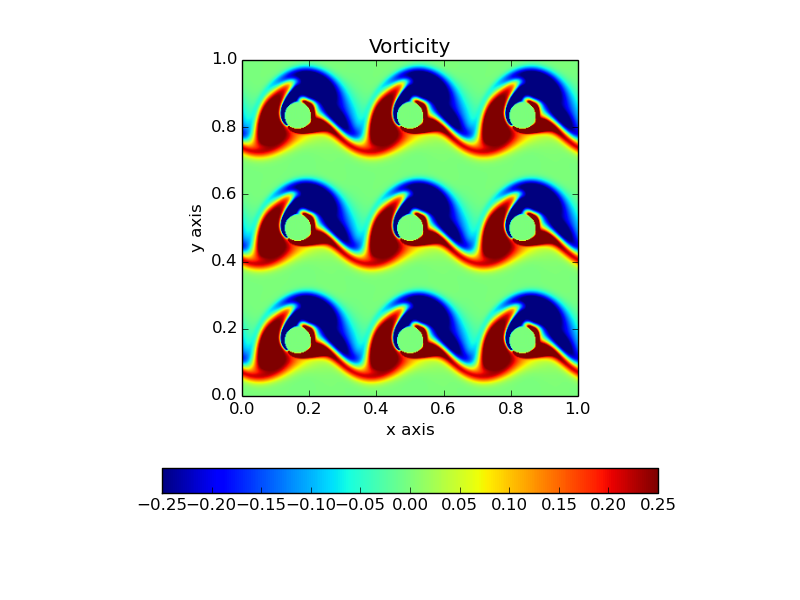
\includegraphics[width=1.1\linewidth, clip=true, trim=1cm 1cm 1cm 1cm]{q1_0004}
  \caption{$n_t = 10000$}
  \label{fig:sub2}
\end{subfigure}
\caption{A figure with two subfigures}
\label{fig:test}
\end{figure}

%----------------------------------------------------------------------------------------
%	QUESTION 2
%----------------------------------------------------------------------------------------
\newpage
\section{}
\textbf{We want to increase the CFL number in order to reduce the cost of the simulation. Using the same second order Adams-Bashforth scheme (\url{itemp=1}), is it possible to run a simulation with a CFL of $0.75$? If yes, generate 4 visualisations of the vorticity field for $n_t = 2500, 5000, 7500, 10000$ and briefly comment on the results in less than 100 words. If not, try to explain why in less than 100 words.}
\newline
\noindent
It is not possible to run the simulations with a CFL of 0.75.

%----------------------------------------------------------------------------------------
%	QUESTION 3
%----------------------------------------------------------------------------------------
\section{}
\textbf{Complete the subroutine \url{rkutta} in which a third-order Runge-Kutta scheme will be used for the me advancement (use the skeleton provided in the code). The scheme is described in sec on 4.3. Run a simulation with the same parameters as in the first simulation but with a $CFL=0.75$ and the newly implemented third-order Runge-Kutta scheme ($itemp=2$, line 38 of the \url{2D_compressible.f90} file)). Generate 4 visualisations of the vorticity field for $nt = 2500, 5000, 7500, 10000$. Briefly comment on the results in less than 100 words and copy-paste the subroutine \url{rkutta} in your report.}

\begin{figure}[htb!]
\centering
\begin{subfigure}{.5\textwidth}
  \centering
  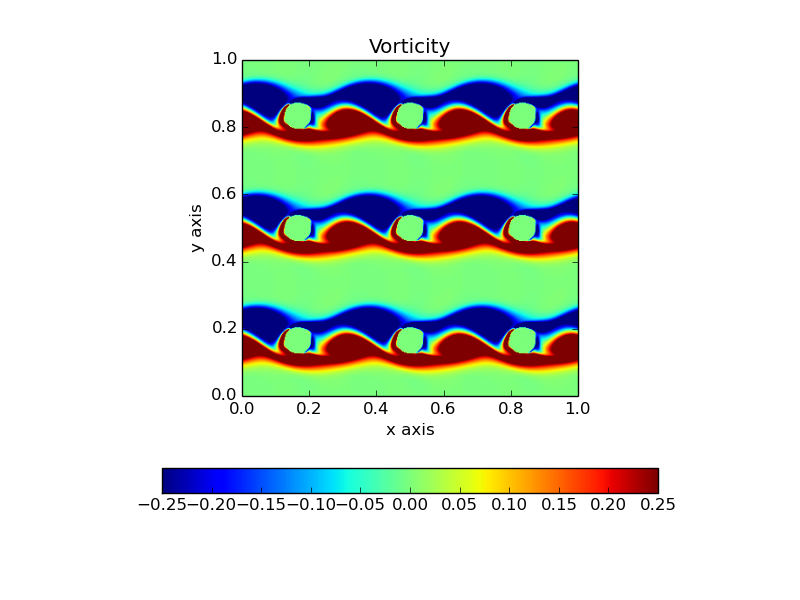
\includegraphics[width=1.1\linewidth, clip=true, trim=1cm 1cm 1cm 1cm]{q3_0001}
  \caption{$n_t = 2500$}
  \label{fig:sub1}
\end{subfigure}%
\begin{subfigure}{.5\textwidth}
  \centering
  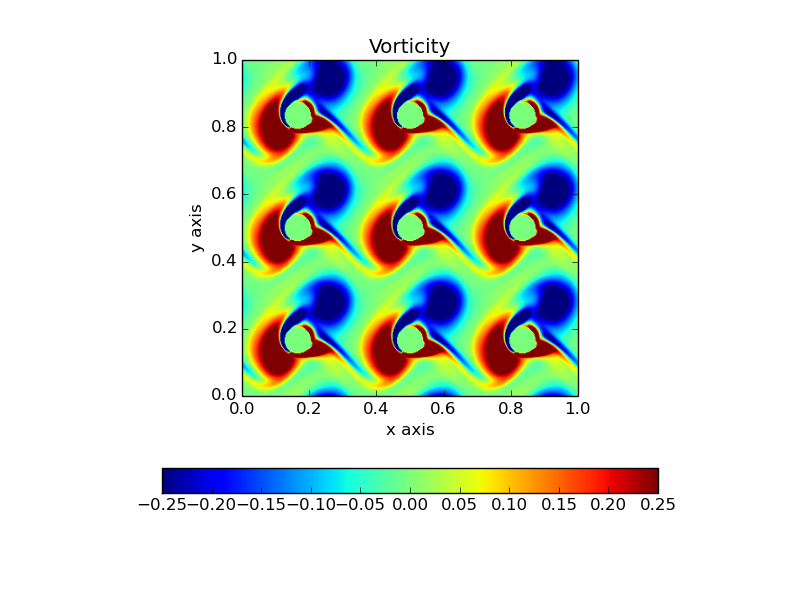
\includegraphics[width=1.1\linewidth, clip=true, trim=1cm 1cm 1cm 1cm]{q3_0002}
  \caption{$n_t = 5000$}
  \label{fig:sub2}
\end{subfigure}
\newline
\begin{subfigure}{.5\textwidth}
  \centering
  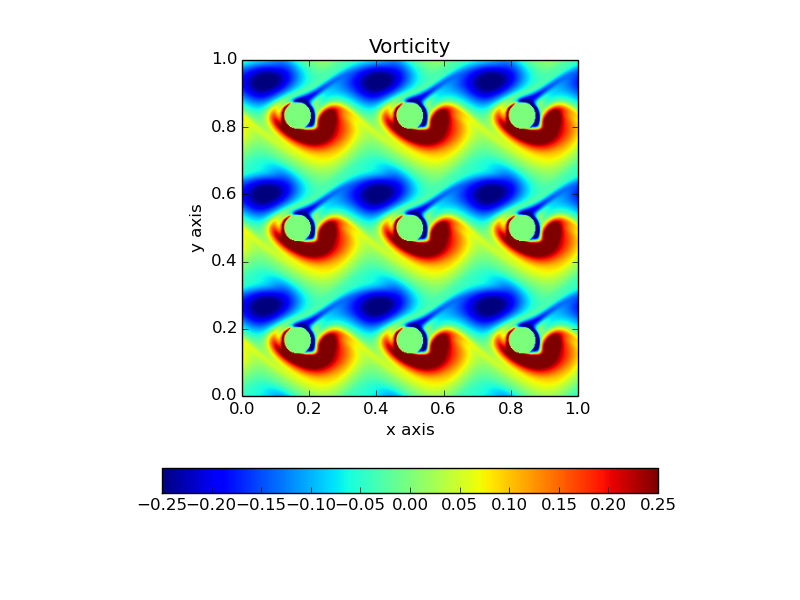
\includegraphics[width=1.1\linewidth, clip=true, trim=1cm 1cm 1cm 1cm]{q3_0003}
  \caption{$n_t = 7500$}
  \label{fig:sub1}
\end{subfigure}%
\begin{subfigure}{.5\textwidth}
  \centering
  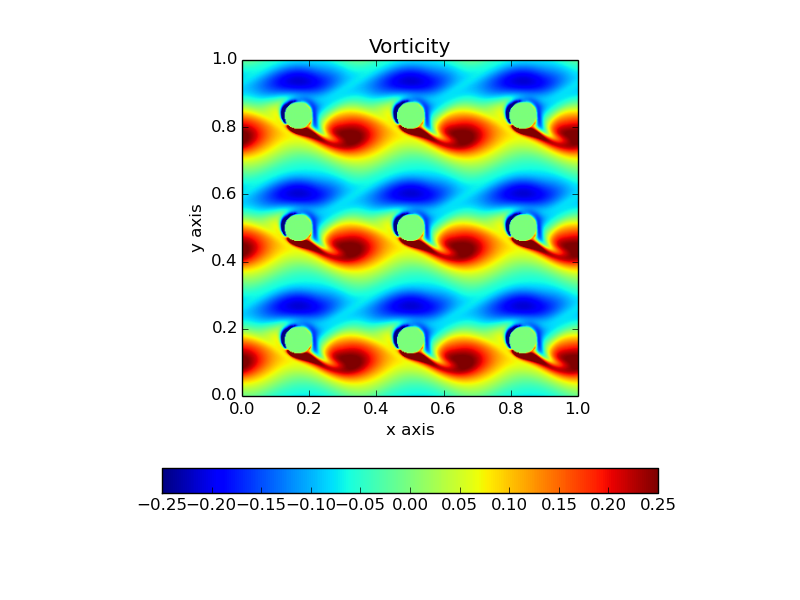
\includegraphics[width=1.1\linewidth, clip=true, trim=1cm 1cm 1cm 1cm]{q3_0004}
  \caption{$n_t = 10000$}
  \label{fig:sub2}
\end{subfigure}
\caption{A figure with two subfigures}
\label{fig:test}
\end{figure}

%----------------------------------------------------------------------------------------
%	QUESTION 4
%----------------------------------------------------------------------------------------
\section{}
\textbf{Instead of circular cylinders, run a simulation using the same parameters as in the first simulation (second order Adams-Bashforth scheme, \url{itemp=1}, $CFL=0.25$) but with square cylinders. The subroutine \url{initl} needs to be modified, in particular for the array \url{eps}. For example, you can define \url{imin},\url{imax},\url{jmin},\url{jmax} where (\url{imin},\url{jmin}) is the bottom left corner of the square, (\url{imin},\url{jmax}) the bottom right corner, (\url{imax},\url{jmin}) the top left corner and (\url{imax},\url{jmax}) the top right corner. The length of the square will be equal to the diameter d of the circular cylinder. Generate 4 visualisations of the vortcity field for $nt = 2500, 5000, 7500, 10000$. Copy-paste the new 2D loop for the square cylinder in your report and briefly comment on the results in less than 50 words.}

%----------------------------------------------------------------------------------------
%	QUESTION 5
%----------------------------------------------------------------------------------------
\section{}
\textbf{We want to use centered fourth-order schemes for the first and second derivatives in the two spatial directions. Write four new subroutines, using the skeletons provided in the code : \url{derix4, deriy4, derxx4} and \url{deryy4}. In the subroutine \url{fluxx}, replace the second-order first and second derivatives with the new fourth-order ones. Then run a simulation with same parameters as the first simulation (question 1) but with the new the fourth-order schemes. Generate 4 visualisations of the vorticity field for $nt = 2500, 5000, 7500, 10000$. Briefly comment on the results and discuss the differences (if any) with the first simulation (question 1) in less than 100 words. Copy-paste the four new subroutines in your report.}

%----------------------------------------------------------------------------------------
%	QUESTION 6
%----------------------------------------------------------------------------------------
\section{}
\textbf{What will happen to the flow if you run the simulation in question 1 for a very long time? Justify your answer in less than 100 words.}

%---------------------------------------------------------------------------------------
%	BIBLIOGRAPHY
% ---------------------------------------------------------------------------------------
\newpage
\bibliographystyle{unsrt}	% in order of appearance
%\bibliographystyle{acm}	% (uses file "plain.bst")
%\bibliographystyle{abbrv}	% (uses file "plain.bst")
%\bibliographystyle{siam}	% (uses file "plain.bst")
%\bibliographystyle{apalike}
\bibliography{/home/fmg215/Documents/latex/myrefs}		% expects file "myrefs.bib"}
%----------------------------------------------------------------------------------------
% END DOCUMENT
%----------------------------------------------------------------------------------------
\end{document}